\chapter{Experimental Comparison and Calibration Targets}

\section{Purpose of the Comparison}

The experimental comparison evaluates whether the COMSOL model reproduces the
direction and approximate shape of observed degradation. It is not an absolute
calibration of device performance or field lifetime. The COMSOL degradation
rate was accelerated to reduce computational time, so simulated seconds and
experimental hours are not directly equivalent.

The comparison uses two reference points: a baseline electronic state and a
degraded light-plus-heat state. The interpretation focuses on PCE reduction,
fill-factor loss, J--V shape, and the mechanism balance among trap growth,
shunting, contact resistance, and mobile-ion redistribution.

\section{Baseline Electronic State}

The experimental X12 baseline has
\begin{equation}
\mathrm{PCE}=14.10\%.
\end{equation}
The COMSOL baseline has
\begin{equation}
\mathrm{PCE}=20.24\%, \qquad
V_{oc}=1.125~\mathrm{V}, \qquad
\mathrm{FF}=83.27\%, \qquad
J_{sc}=21.61~\mathrm{mA/cm^2}.
\end{equation}
The COMSOL baseline is more ideal than the experiment. This mismatch is
expected for an initial physics model because idealized contacts, uniform
or simplified photogeneration, one-dimensional geometry, and literature-based material
parameters tend to reduce nonradiative and resistive losses. The baseline
therefore provides a reference for mechanism studies, not a fully calibrated
absolute representation of the experimental device.

The calibration target is clear: absolute baseline performance requires
adjusting absorber generation, transport-layer barriers, trap density, surface
recombination, contact resistance, and shunt leakage so that $V_{oc}$,
$J_{sc}$, FF, and PCE all match the same device before degradation parameters
are interpreted physically.

\section{Degraded Light-Plus-Heat State}

The experimental device after 24 h light-plus-heat stress has
\begin{equation}
\mathrm{PCE}=10.05\%.
\end{equation}
The accelerated COMSOL light-plus-heat case after 60 s has
\begin{equation}
\mathrm{PCE}=10.85\%, \qquad
V_{oc}=1.021~\mathrm{V}, \qquad
\mathrm{FF}=53.46\%, \qquad
J_{sc}=19.87~\mathrm{mA/cm^2}.
\end{equation}
The simulated degradation direction is consistent with the experimental trend:
PCE decreases, FF decreases strongly, and the J--V curve develops a degraded
knee. The simulated $J_{sc}$ also decreases, which is consistent with stronger
recombination or reduced effective generation.

The agreement is qualitative. The comparison supports the use of trap growth,
shunt leakage, contact resistance, and mobile-ion redistribution as candidate
mechanisms, but it does not uniquely identify their relative weights. The
accelerated timescale, baseline mismatch, and incomplete validation of
ion--trap coupling prevent a calibrated lifetime claim.

\section{Stress-Specific Comparison Targets}

The Research Explorer comparison package adds stress-specific experimental
targets for light-only, heat-only, and light-plus-heat exposure. These figures
combine experimental metric scatter, median trends, and representative J--V
curves with the current COMSOL comparison cases. They are used here as
calibration targets rather than as fitted validation, because the experimental
sets differ in stress duration, light intensity, sample count, and starting
device performance.

\begin{figure}[H]
\centering
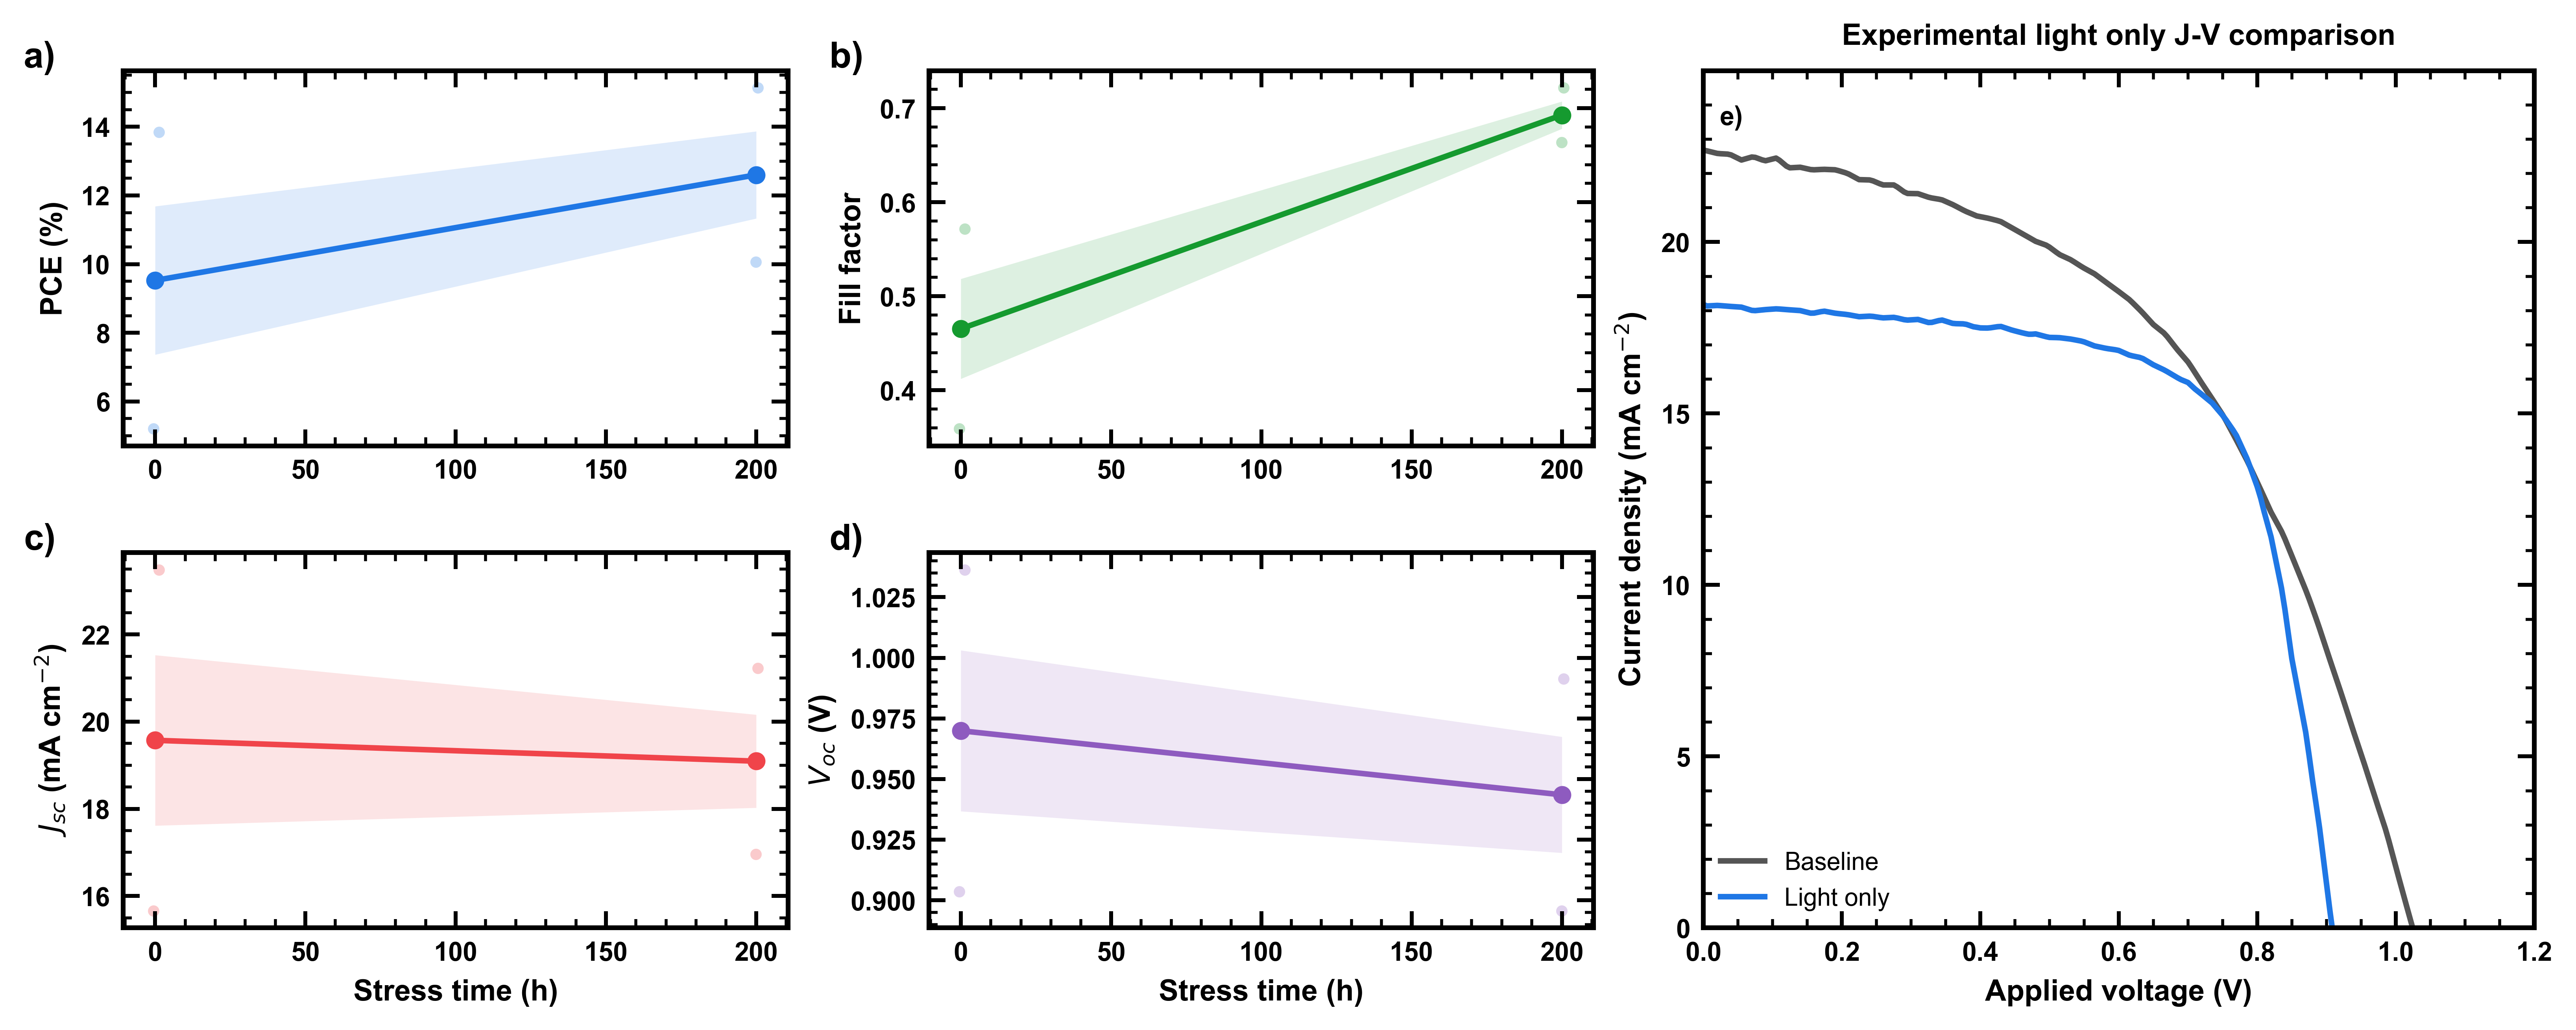
\includegraphics[width=\textwidth]{outputs/figures/comsol_experimental_comparison/xrf_light_only_comsol_comparison.png}
\caption{Light-only experimental comparison used as a COMSOL calibration
target. The light-only endpoint shows a much milder degradation signature than
the coupled light-plus-heat case, so light-driven trap and transport changes
should remain weaker than the combined stress channel.}
\label{fig:xrf_light_only_comsol_comparison}
\end{figure}

\begin{figure}[H]
\centering
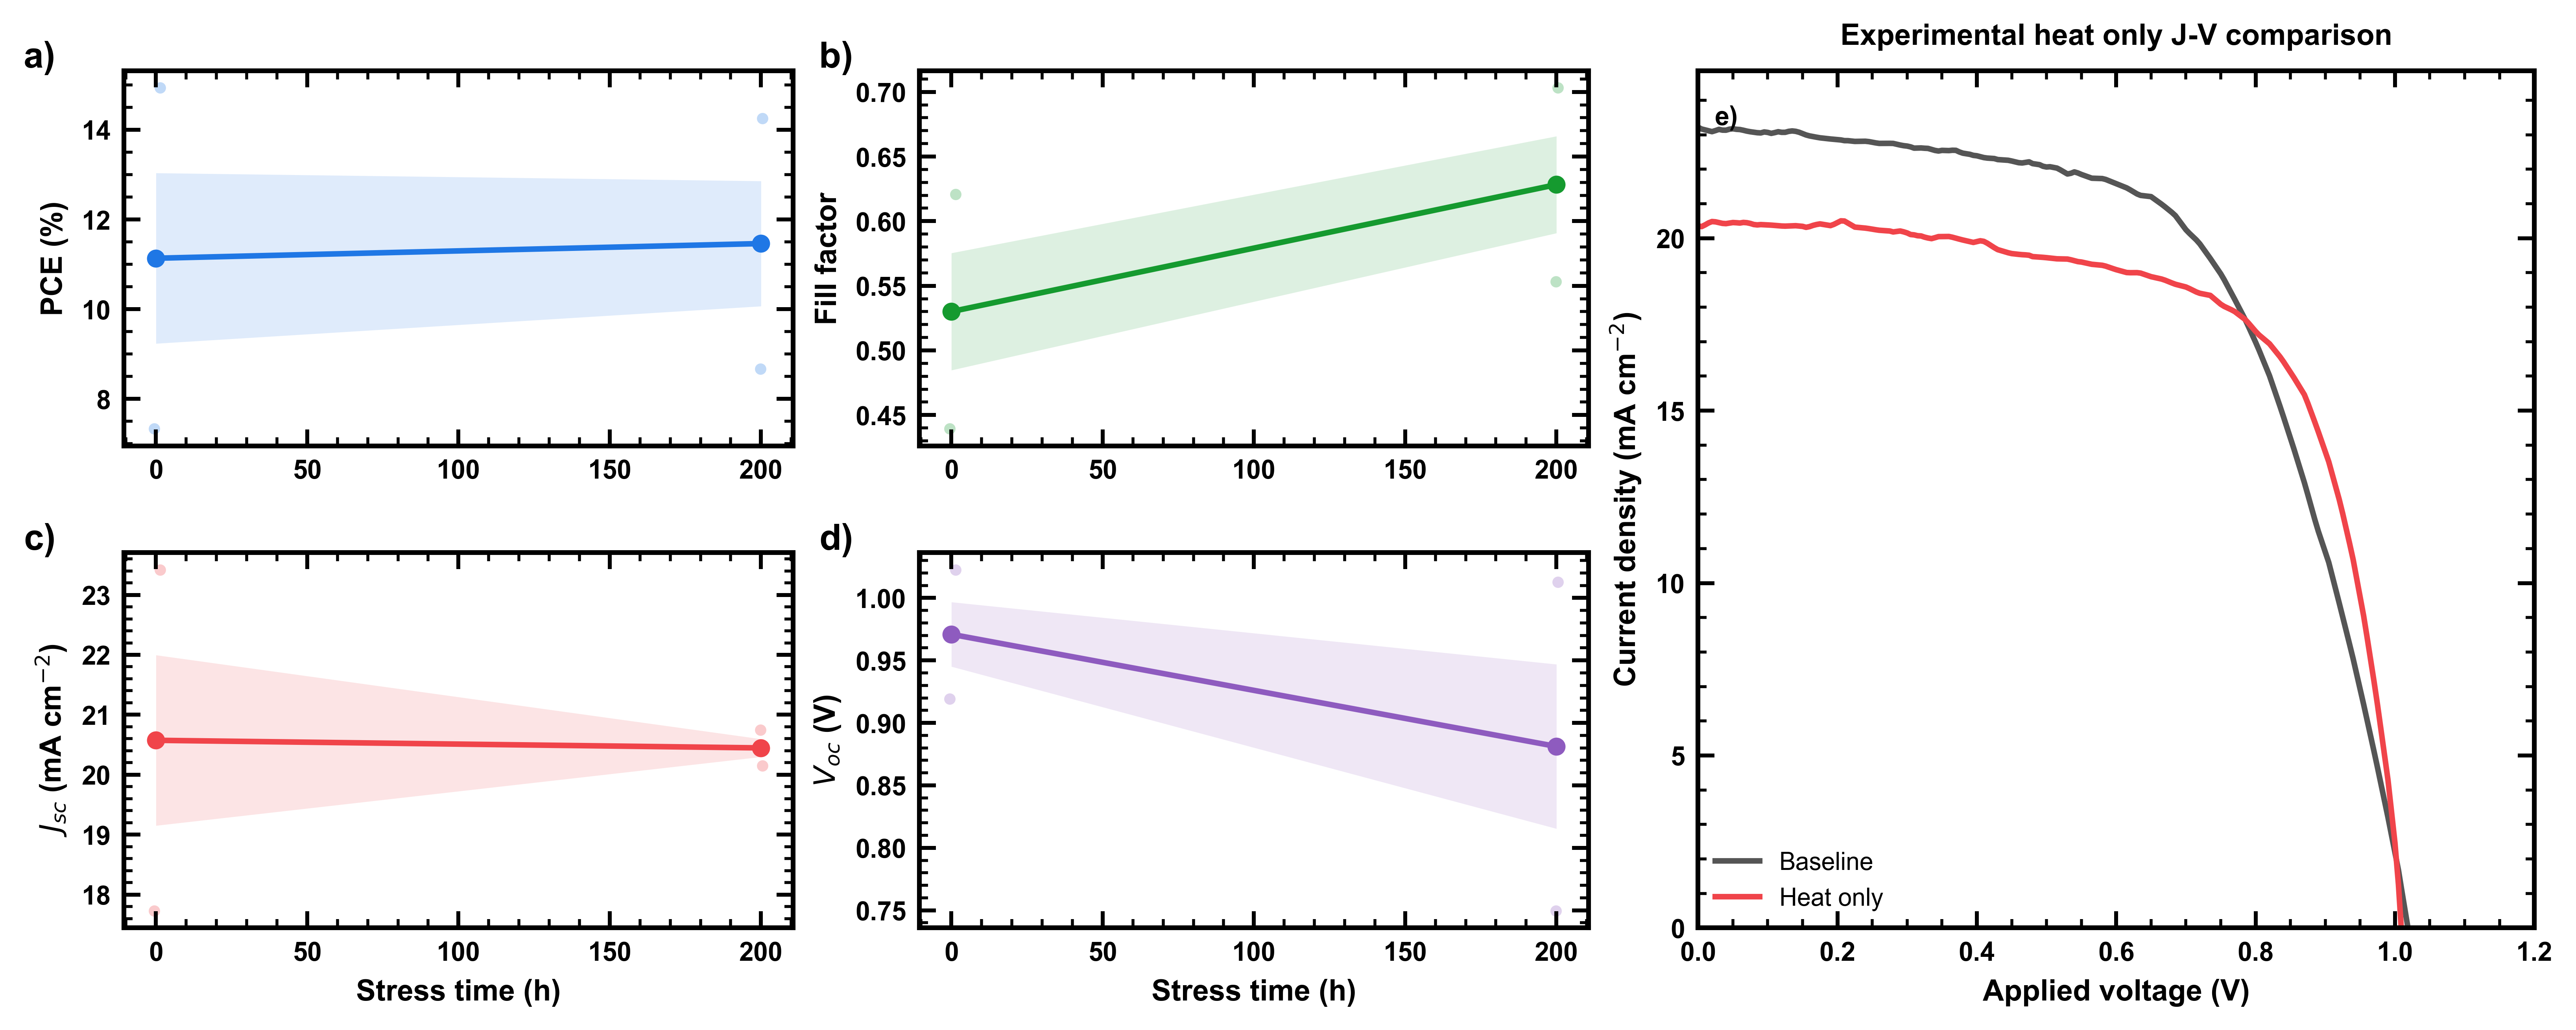
\includegraphics[width=\textwidth]{outputs/figures/comsol_experimental_comparison/xrf_heat_only_comsol_comparison.png}
\caption{Heat-only experimental comparison used as a COMSOL calibration
target. This case isolates the thermal contribution and constrains the model so
that heat by itself does not reproduce the full coupled light-plus-heat
degradation pathway.}
\label{fig:xrf_heat_only_comsol_comparison}
\end{figure}

\begin{figure}[H]
\centering
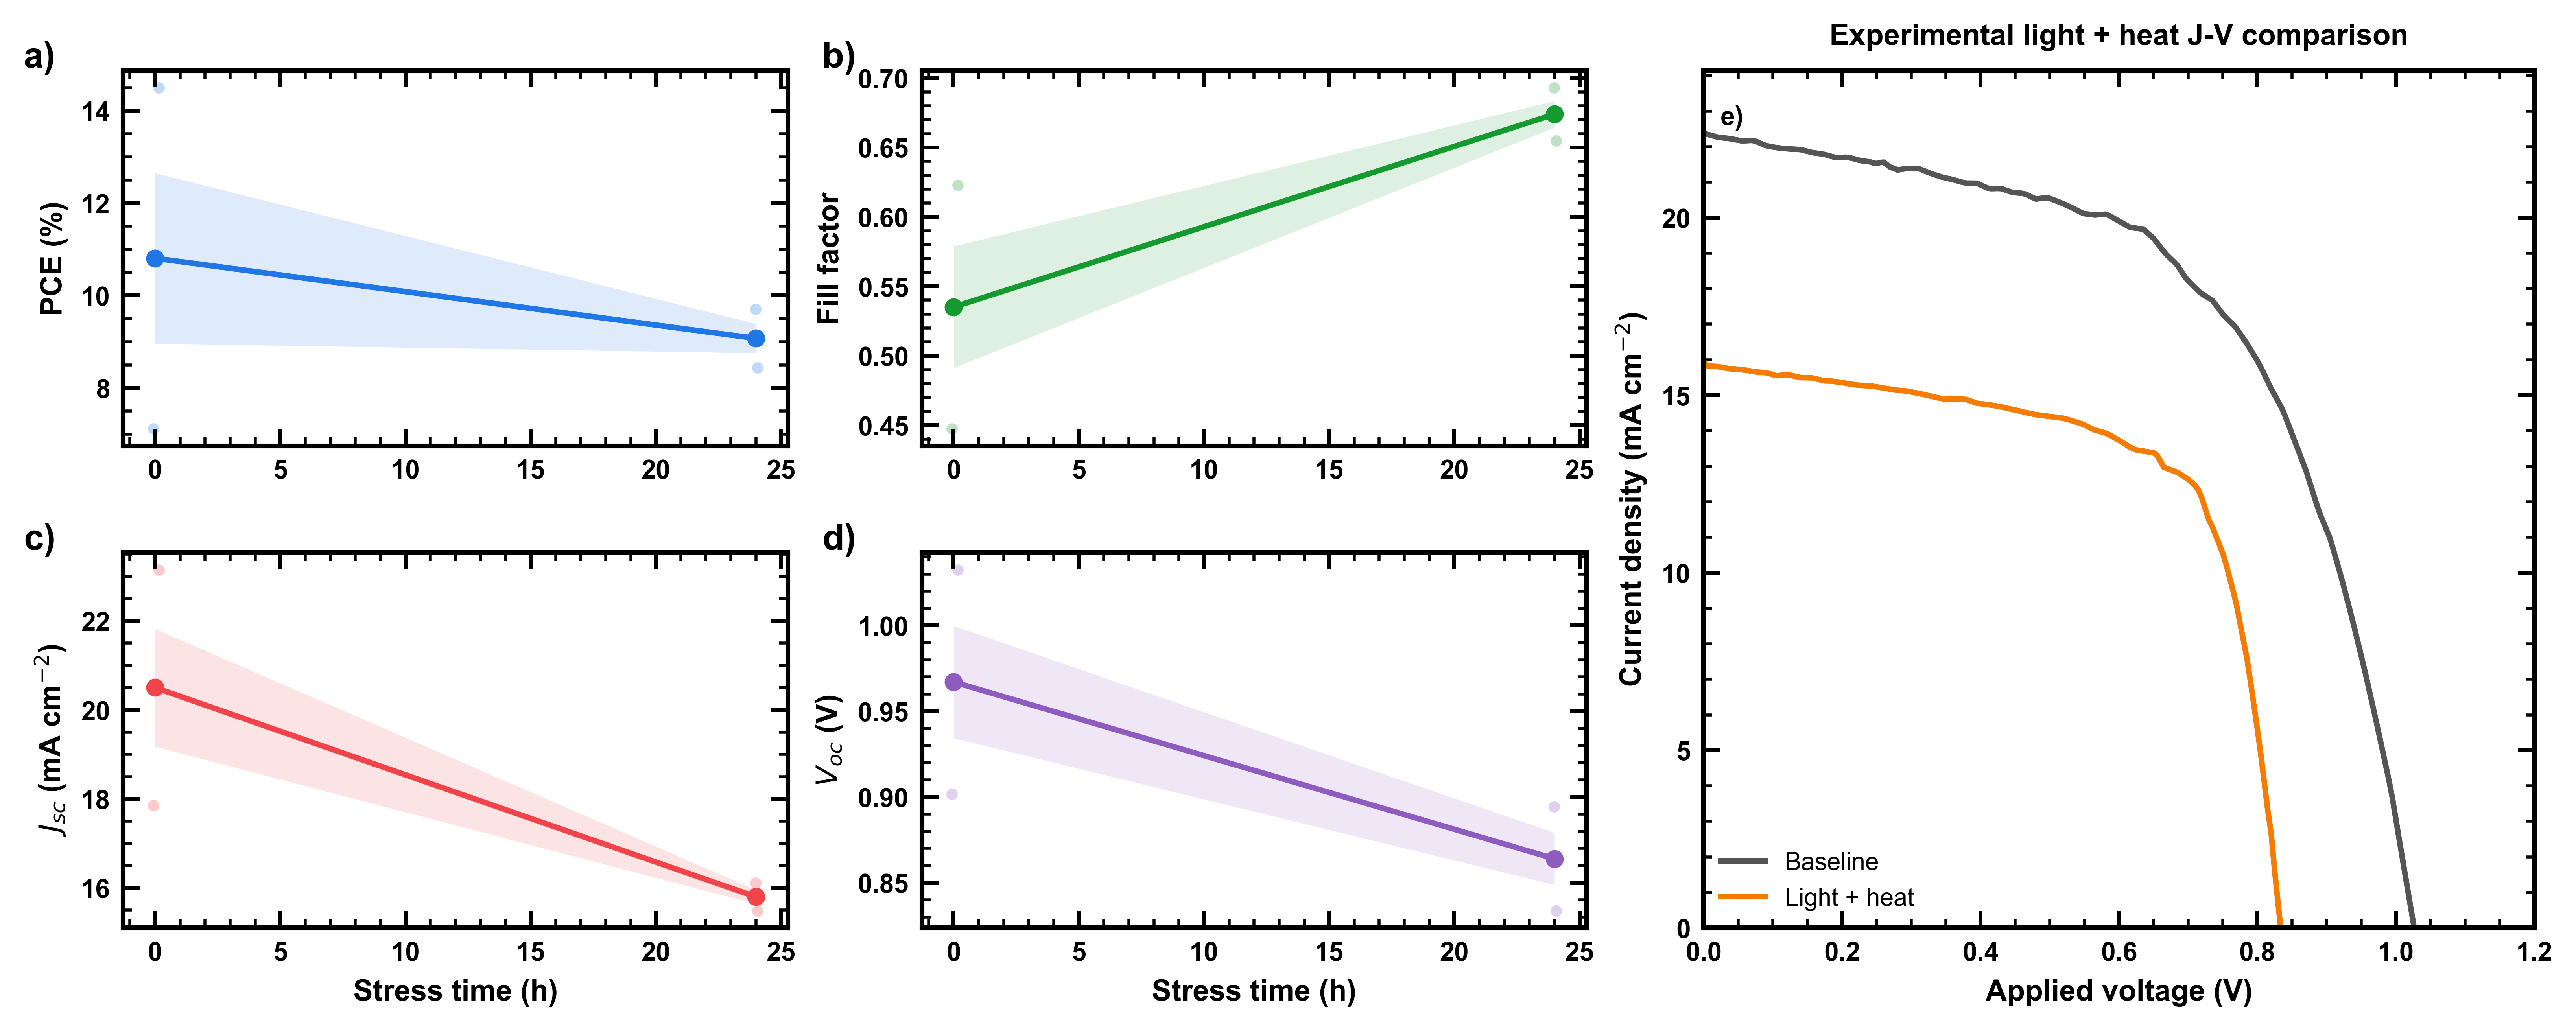
\includegraphics[width=\textwidth]{outputs/figures/comsol_experimental_comparison/xrf_light_heat_comsol_comparison.png}
\caption{Light-plus-heat experimental comparison used as a COMSOL calibration
target. The coupled stress condition produces the strongest endpoint loss in
the matched XRF stress matrix and is therefore the primary target for tuning
combined recombination, transport, and leakage changes.}
\label{fig:xrf_light_heat_comsol_comparison}
\end{figure}

\begin{figure}[H]
\centering
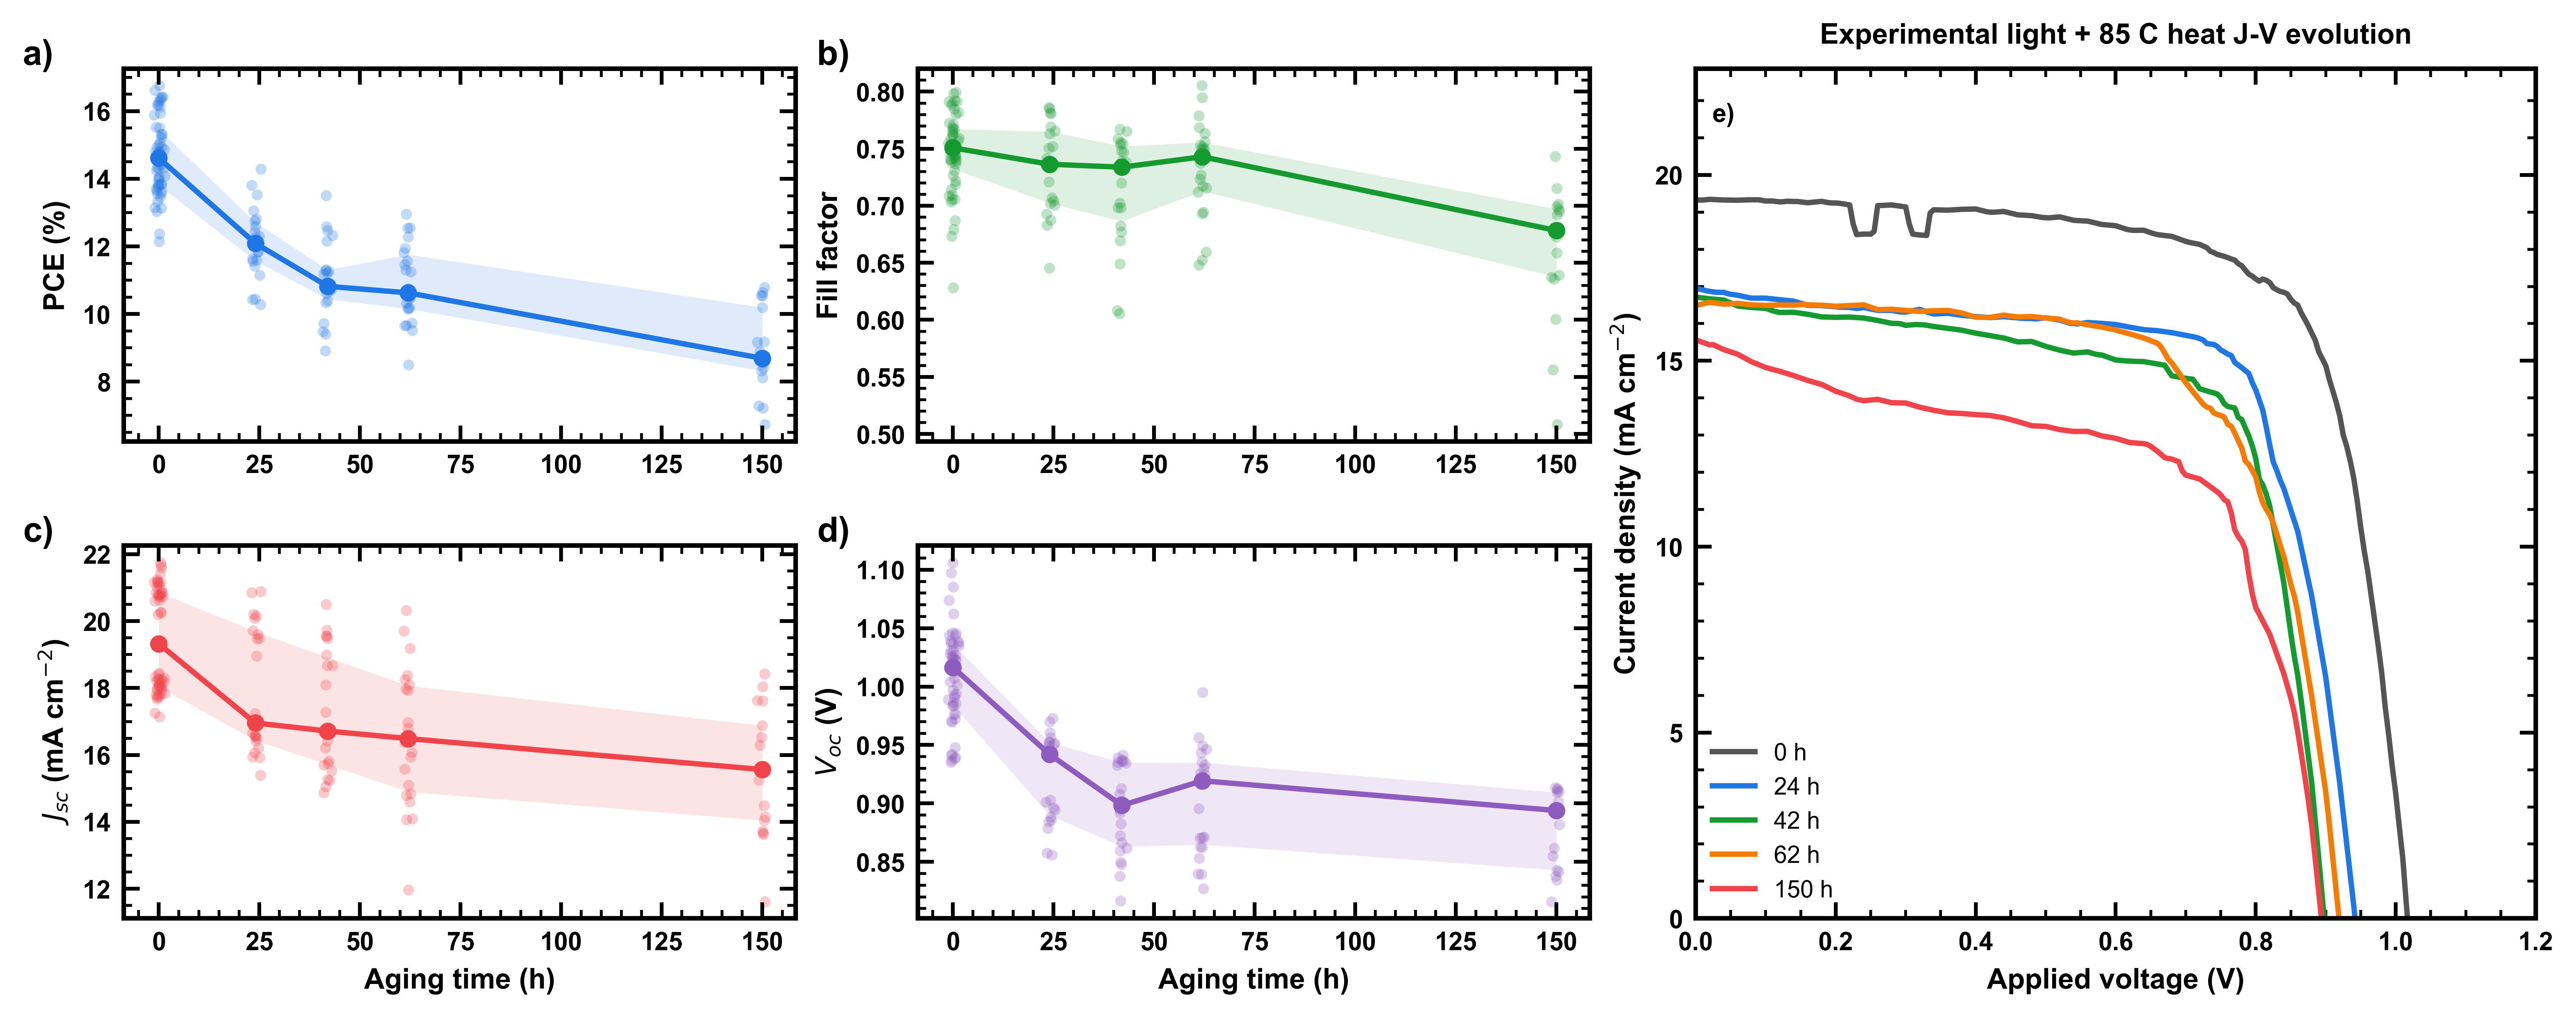
\includegraphics[width=\textwidth]{outputs/figures/comsol_experimental_comparison/exp3_lh_85c_comsol_comparison.png}
\caption{Light plus 85~$^\circ$C aging comparison from the Exp3 dataset. The
larger time series shows sustained performance loss, with median PCE decreasing
from about 14.6\% at 0 h to about 8.7\% at 150 h, and provides the strongest
multi-time-point target for coupled degradation calibration.}
\label{fig:exp3_lh_85c_comsol_comparison}
\end{figure}

Together, these comparisons show why the degradation model should not be
calibrated only to PCE. Light-only and heat-only endpoints show milder or
partially compensating changes in the electronic metrics, while coupled
light-plus-heat exposure produces a more consistent loss in current, voltage,
fill factor, and J--V curve shape. A useful calibration must therefore match
both the metric trajectories and the stress-dependent J--V shape.

\section{Mechanism Balance}

Several mechanisms can produce similar PCE loss. Increased trap density lowers
carrier lifetimes through the SRH relation and reduces $V_{oc}$. Decreased
shunt resistance increases leakage near short circuit and reduces FF. Increased
series resistance rounds the high-forward-bias knee and reduces FF with limited
direct effect on $V_{oc}$. Mobile-ion redistribution changes the internal
space-charge profile through Eq.~\ref{eq:rho_ion}, shifting band bending and
creating scan-history dependence.

The degraded comparison therefore cannot be interpreted from PCE alone. A
calibrated fit must match the full J--V shape, forward/reverse scan separation,
voltage-dependent slope, and time evolution. Impedance, transient photocurrent,
capacitance, photoluminescence, and ion-current measurements would reduce the
non-uniqueness by constraining mobile-ion and recombination parameters
\cite{SchmidtPRX_2025,Elhorst_2025,SchmidtACS_2025}.

\section{Calibration Needs}

The model needs four calibration steps before it can support device-specific
lifetime prediction:
\begin{enumerate}
\item match the pristine J--V curve in absolute $V_{oc}$, $J_{sc}$, FF, and
PCE;
\item calibrate the accelerated degradation factors against measured aging
times;
\item separate the relative contributions of trap loss, shunt loss, contact
resistance, photogeneration loss, and surface recombination; and
\item validate the mobile-ion distribution and ion--trap coupling with
ion-sensitive or hysteresis-sensitive measurements.
\end{enumerate}

Until those steps are complete, the COMSOL model is best interpreted as a
physics-based mechanism-separation platform rather than a final lifetime
prediction tool.

\section{Architecture-Specific Calibration Context}

The laboratory program includes both
ITO-glass/NiO$_x$/perovskite/C$_{60}$/BCP/Ag devices and bilayer
ITO-glass/NiO$_x$/MeO-2PACz/perovskite/C$_{60}$/BCP/Ag devices. The
presentation and this thesis use the bilayer p-i-n architecture as the primary
device truth. Baseline, light-only, heat-only, light-plus-heat, glovebox
control, and dark-recovery measurements should therefore be grouped by
architecture before parameter fitting.

Literature and laboratory comparisons indicate that different absorber and
contact architectures need not degrade through the same dominant electrical
signature. A strong $J_{sc}$ decrease suggests generation or collection loss,
a dominant FF decrease suggests contact or shunt loss, and a large $V_{oc}$
decrease suggests stronger recombination. These are diagnostic hypotheses, not
unique assignments. The model should fit the complete J--V curve and supporting
ion-sensitive or optical measurements before attributing a measured trend to
one channel.
